\chapter{Basics of Digital Circuits}
\label{ch:digital}
Until now, we considered a transistor mostly as an analog element: by applying a voltage at the input (e.g. the base or gate), we generate a continuous and varying current which in turn induces an output voltage that changes in a continuous fashion. In this part, we consider a transistor as a controllable switch: the input signal is a low or high voltage, and the output voltage will be as well.\\
An npn transistor behaves as a closed switch when $v_{BE} > 0.6$ V. In that case there will be a lot of current $i_C$ for a small $v_{CE}$ and the transistor is in the saturation region. When $v_{BE} < 0.6$ V, there will be (almost) no current and the transistor is in the cut-off region. It acts as an open switch. Obviously, an pnp is open or closed when $v_{EB} < 0.6$ and $v_{EB} > 0.6$, respectively.\\
The situation is similar for a MOSFET: an n-channel MOSFET behaves as an closed switch when $v_{GS} > V_T$. The transistor will operate in the linear region - especially there where the curves are steep and the resistance is small. On the other hand, when $v_{GS} < V_T$, no current can flow and the MOSFET is an open switch. For a PMOS, the criterion is $v_{SG} > V_T$ (closed) or  $v_{SG} < V_T$ (open).

\begin{minipage}{.5\textwidth}
	\centering
	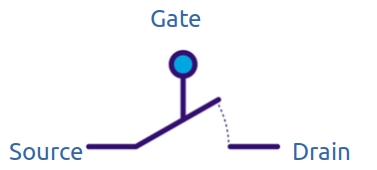
\includegraphics[width=6cm]{figures/ch13/switch.jpg}
	\captionof{figure}{}
	\label{fig:switch}
\end{minipage}%
\begin{minipage}{.5\textwidth}
	\centering
	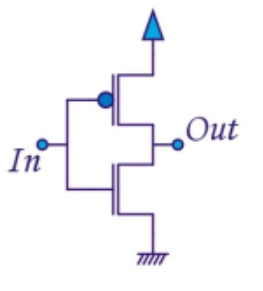
\includegraphics[width=4cm]{figures/ch13/not_gate.jpg}
	\captionof{figure}{}
	\label{fig:not_gate}
\end{minipage}

When we put a PMOS on top of an NMOS, we create a NOT-gate, as in figure \ref{fig:not_gate}. If the input is at a low voltage (a logical "0"), $V_{GS, N} < V_T$ and $V_{SG, P} > V_T$, so the bottom transistor is an open switch and the top one is closed. This means that the output is connected to the supply, and it is high ("1"). If the input is high, the top transistor will not conduct and is an open switch, and the output is connected to the ground via the closed NMOS. Hence the output is low. From this analysis, we can construct the truth table for this gate:\\



\begin{minipage}{.2\textwidth}
	\begin{center}
		\begin{tabular}{|c|c|}
			\hline
			In  & Out \\
			\hline\hline
			0 & 1 \\
			\hline
			1 & 0 \\
			\hline
		\end{tabular}
	\end{center}
\end{minipage}%
\begin{minipage}{.8\textwidth}
	Because the output is the opposite of the input, this is called a NOT-gate. The circuit is constructed such that both "switches" can never be closed at the same time. We will come back to this property in chapter \ref{ch:logic_gates}.\\
\end{minipage}

We must however keep in mind that a logical gate is in essence an analog circuit, and the output $v_{out}$ varies in a continuous way as the input voltage $v_{in}$ increases, as in figure \ref{fig:not_gate2b}. We can analyze this behavior with the help of figure \ref{fig:not_gate3}, where we see the $i_{DS} - v_{DS}$ characteristic the NMOS, and superimposed the $i_{SD} - v_{SD}$ curve of the PMOS. We can do this because $i_{DS} = i_{SD} = i$ and $v_{DS} + v_{SD} = E$.\\

\begin{minipage}{.5\textwidth}
	\centering
	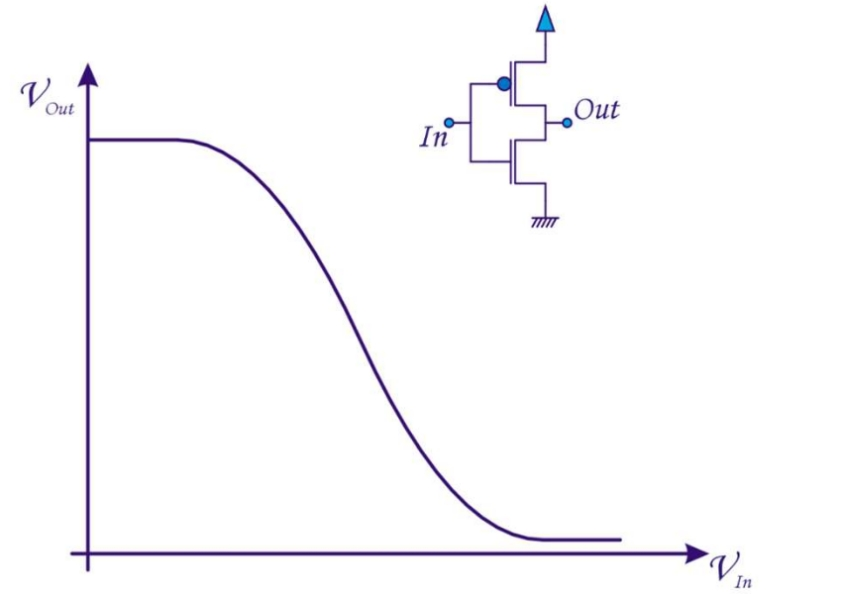
\includegraphics[width=8cm]{figures/ch13/not_gate2.jpg}
	\captionof{figure}{}
	\label{fig:not_gate2b}
\end{minipage}%
\begin{minipage}{.5\textwidth}
	\centering
	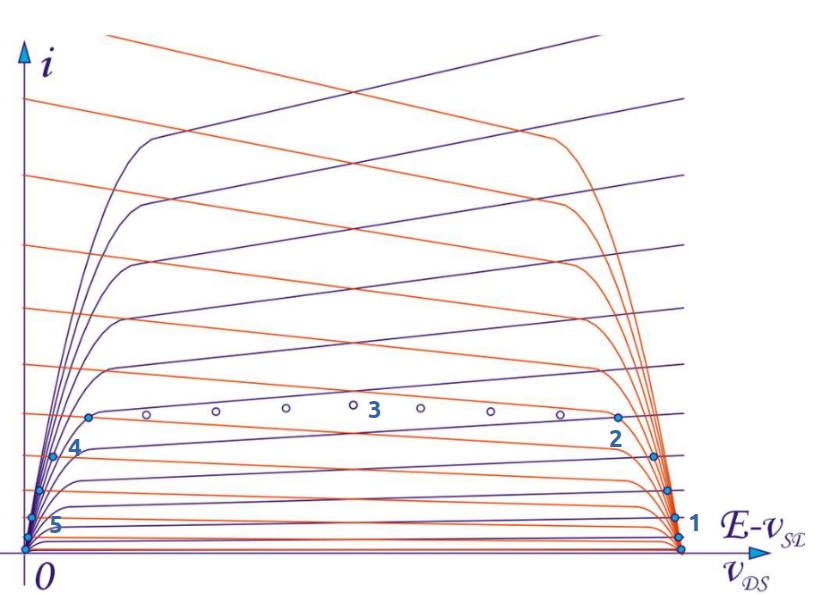
\includegraphics[width=8cm]{figures/ch13/not_gate3.jpg}
	\captionof{figure}{}
	\label{fig:not_gate3}
\end{minipage}

If $v_{IN}$ is small, the NMOS is in cut-off , while the PMOS is in deep triode (linear) region because it wants to draw lots of current but it can't. We are in point \Circled{1}, and the output voltage $v_{out} = v_{DS}$ is high. As $v_{IN}$ increase and becomes $v_{IN} = v_{T, N}$, the NMOS will turn on and, because $v_{DS}$ is high, will be in saturation. So we will be on a higher blue line which represents $i_{DS} = f(v_{DS})$ for a fixed $v_{GS, N}$. At the same time, $v_{SG, P}$ decreases so we will be on lower red line. The net result is that the intersection point (the dot) ¨moves slightly to the left and $V_{out}$ starts to decrease slightly \Circled{2}. At a certain moment, the PMOS leaves the linear region because $v_{SD} = E - v_{out}$ becomes large enough (i.e. $v_{SD} > v_{SG,P} - V_{T,P}$). From that moment on, there will be a significant current in the gate, and the output will decrease fast with increasing $v_{IN}$. We are in point \Circled{3} of figure \ref{fig:not_gate2}. This continues until the NMOS goes in the linear region \Circled{4}, where the current will decrease, and finally the input voltage becomes too high to create a channel in the PMOS: $v_{SG, P} < V_{T,P}$: there is no more current and the output is low \Circled{5}. \\
This also means also that the input-output characteristic of the gate will depend on the I-V characteristics of the transistor, and consequently there will be a lot of variance between these curves. To accommodate this, the manufacturer will define certain threshold voltages to ensure proper operation of the gate, as in figure \ref{fig:digital_thresholds}:

\begin{figure}[h!]
	\centering
	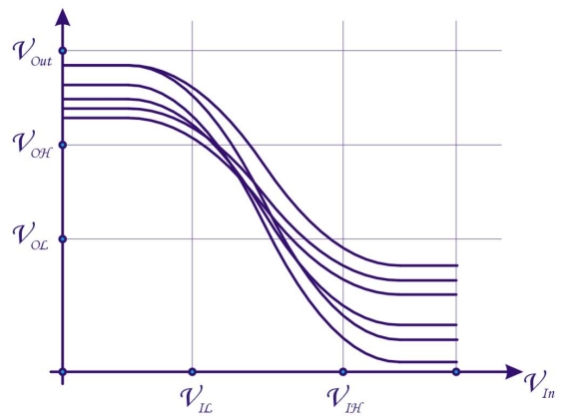
\includegraphics[height=6cm]{figures/ch13/digital_thresholds.jpg}
	\caption{}
	\label{fig:digital_thresholds}
\end{figure}

\begin{itemize}
	\item $V_{IH}$ : Minimum input voltage so that the output is guaranteed to be low,
	\item $V_{IL}$ : Maximum input voltage so that the output is guaranteed to be high,
	\item $V_{OH}$ : Minimum gate output when the gate generates a logic high
	\item $V_{OL}$ : Maximum gate output when the gate generates a logic low
\end{itemize}

A specific technology will work only if $V_{IL} > V_{OL}$ and $V_{IH} < V_{OH}$, because only then can we put multiple gates in cascade and still guarantee their proper operation.\\
There exist different logic families:
\begin{itemize}
	\item DTL (Diode-Transistor Logic)
	\item TTL (Transistor-Transistor Logic)
	\item ECL (Emitter-Coupled Logic)
	\item CMOS (Complementary MOS)
	\item \ldots
\end{itemize}
We will mostly work with CMOS where both NMOS and PMOS devices are used in the same substrate, but we'll also study other technologies in chapter \ref{ch:alternative}. Each family has its own nominal power supply and threshold voltages $V_{IH}, V_{IL}, V_{OH}$ and $V_{OL}$. It is therefore not recommended to mix different logical families. If this is required, you must check that $V_{IL} > V_{OL}$ and $V_{IH} < V_{OH}$, or use adapter gates.

\chapter{Logic Gates}
\label{ch:logic_gates}
\section{Basic Logic Gates}

We already saw the NOT-gate in the previous chapter, together with its truth table. From boolean logic, we also know that we can create gates with more than one input, like the well-known AND- and OR-gates. These gates, together with their symbol are shown on the next page. We can also combine a NOT-gate with an AND- or OR-gate, to obtain a NAND and a NOR-gate. This may seem cursory, but in actuality it is easier to produce a NAND or NOR-gate in CMOS than a simple AND- or OR-gate. Furthermore, it can be shown that these gates are universal: any combinatorial circuit can be realized with only NAND or NOR-gates.\\
Another specific gate is the eXclusive OR or XOR-gate: its output is only high when exactly one of its inputs is high, and zero otherwise. This operation is also represented by the symbol $a \; \oplus  \;  b $.\\
Finally, a gate that produces the same logical output as its input is a buffergate, as shown in figure \ref{fig:buffer_gate} together with its truth table, which is trivial. This gate must be used to interface with analog circuits, i.e. every time you receive a binary input somewhere, or when a binary output has to drive a (large) load. They should also be used when going from one logic family to another, like when you use TTL to drive a CMOS camera.

\begin{figure}[h!]
	\centering
	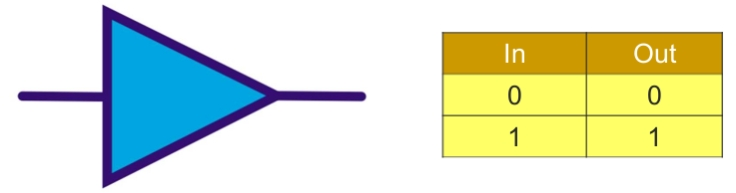
\includegraphics[width=10cm]{figures/ch13/buffer_gate.jpg}
	\caption{}
	\label{fig:buffer_gate}
\end{figure}

In this chapter, we will use these gates to construct arbitrary boolean expressions. We'll see what Karnaugh mapping is and how it can be used to simplify expressions, and how these logic functions can be implemented with CMOS gates. We'll see two examples of this design procedure: the implementation of a digital multiplexer or MUX, and the implementation of an adder circuit.

\newpage
% NOT
\begin{minipage}{.4\textwidth}
	\centering
	
\includegraphics[width=4cm]{figures/ch13/symbol_not.jpg}
	%\captionof{figure}{}
	\label{fig:not_gate2}
\end{minipage}%
\begin{minipage}{.2\textwidth}
	NOT a = $\overline{a}$
\end{minipage}%
\begin{minipage}{.4\textwidth}
	%\begin{center}
		\begin{tabular}{|c|c|}
			\hline
			In  & Out \\
			\hline\hline
			0 & 1 \\
			\hline
			1 & 0 \\
			\hline
		\end{tabular}
	%\end{center}
\end{minipage}

% AND
\begin{minipage}{.4\textwidth}
	\centering
	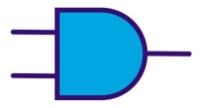
\includegraphics[width=4cm]{figures/ch13/symbol_and.jpg}
	%\captionof{figure}{}
	\label{fig:symbol_and}
\end{minipage}%
\begin{minipage}{.2\textwidth}
	a AND b = $a\cdot b$
\end{minipage}%
\begin{minipage}{.4\textwidth}
	%\begin{center}
	\begin{tabular}{|c|c|c|}
		\hline
		a & b  & $a\cdot b$ \\
		\hline\hline
		0 & 0 & 0 \\
		\hline
		0 & 1 & 0 \\
		\hline
		1 & 0 & 0 \\
		\hline
		1 & 1 & 1 \\
		\hline
	\end{tabular}
	%\end{center}
\end{minipage}

% OR
\begin{minipage}{.4\textwidth}
	\centering
	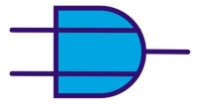
\includegraphics[width=4cm]{figures/ch13/symbol_or.jpg}
	%\captionof{figure}{}
	\label{fig:symbol_or}
\end{minipage}%
\begin{minipage}{.2\textwidth}
	a OR b = $a + b$
\end{minipage}%
\begin{minipage}{.4\textwidth}
	%\begin{center}
	\begin{tabular}{|c|c|c|}
		\hline
		a & b  & $a + b$ \\
		\hline\hline
		0 & 0 & 0 \\
		\hline
		0 & 1 & 1 \\
		\hline
		1 & 0 & 1 \\
		\hline
		1 & 1 & 1 \\
		\hline
	\end{tabular}
	%\end{center}
\end{minipage}

% XOR
\begin{minipage}{.4\textwidth}
	\centering
	
\includegraphics[width=4cm]{figures/ch13/symbol_xor.jpg}
	%\captionof{figure}{}
	\label{fig:symbol_xor}
\end{minipage}%
\begin{minipage}{.2\textwidth}
	a XOR b \\= $a\overline{b} + \overline{a}b$
\end{minipage}%
\begin{minipage}{.4\textwidth}
	%\begin{center}
	\begin{tabular}{|c|c|c|}
		\hline
		a & b  & $a\overline{b} + \overline{a}b$ \\
		\hline\hline
		0 & 0 & 0 \\
		\hline
		0 & 1 & 1 \\
		\hline
		1 & 0 & 1 \\
		\hline
		1 & 1 & 0 \\
		\hline
	\end{tabular}
	%\end{center}
\end{minipage}

% NAND
\begin{minipage}{.4\textwidth}
	\centering
	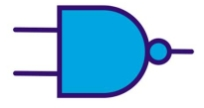
\includegraphics[width=4cm]{figures/ch13/symbol_nand.jpg}
	%\captionof{figure}{}
	\label{fig:symbol_nand}
\end{minipage}%
\begin{minipage}{.2\textwidth}
	a NAND b \\= $\overline{a \cdot b}$
\end{minipage}%
\begin{minipage}{.4\textwidth}
	%\begin{center}
	\begin{tabular}{|c|c|c|}
		\hline
		a & b  & $\overline{a \cdot b}$ \\
		\hline\hline
		0 & 0 & 1 \\
		\hline
		0 & 1 & 1 \\
		\hline
		1 & 0 & 1 \\
		\hline
		1 & 1 & 0 \\
		\hline
	\end{tabular}
	%\end{center}
\end{minipage}

% NOR
\begin{minipage}{.4\textwidth}
	\centering
	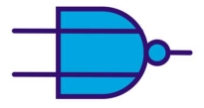
\includegraphics[width=4cm]{figures/ch13/symbol_nor.jpg}
	\captionof{figure}{}
	\label{fig:symbol_nor}
\end{minipage}%
\begin{minipage}{.2\textwidth}
	a NOR b \\= $\overline{a + b}$
\end{minipage}%
\begin{minipage}{.4\textwidth}
	%\begin{center}
	\begin{tabular}{|c|c|c|}
		\hline
		a & b  & $\overline{a + b}$ \\
		\hline\hline
		0 & 0 & 1 \\
		\hline
		0 & 1 & 0 \\
		\hline
		1 & 0 & 0 \\
		\hline
		1 & 1 & 0 \\
		\hline
	\end{tabular}
	%\end{center}
\end{minipage}

\section{Complex Logic Gates}
Any logic function $F$ can be defined with its truth table, where every combination of the inputs is enumerated together with the output. For a system with $N$ inputs, this table has $2^N$ input lines\footnote{The total number of possible truth tables for systems with $N$ inputs is $2^{2^N}$}. As an example, consider the table in figure \ref{fig:truth_table}.
\begin{figure}[h!]
	\centering
	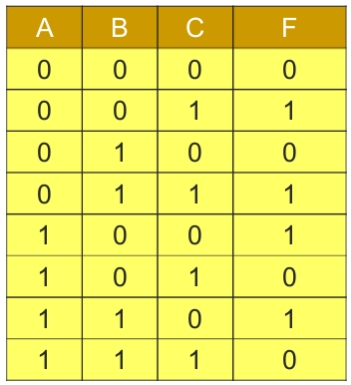
\includegraphics[width=6cm]{figures/ch13/truth_table.jpg}
	\caption{}
	\label{fig:truth_table}
\end{figure}
Equivalently, we can represent a logic function by a Boolean expression. This can be done in two ways:
\begin{enumerate}
	\item \textbf{Sum-of-Products}: only consider the rows with output equal to $1$\\
	$F = \overline{A} \cdot \overline{B}  \cdot  C + \overline{A} \cdot  B  \cdot  C + A  \cdot \overline{B}  \cdot \overline{C} + \overline{A}  \cdot B  \cdot C $
	\item \textbf{Product-of-Sums}: only consider the rows with output equal to $0$\\
	$F = (A + B + C) \cdot (A + \overline{B} + C) \cdot (\overline{A} + B + \overline{C}) \cdot (\overline{A} + \overline{B} + \overline{C}) $
\end{enumerate} 

These methods are equivalent: 
\begin{align*}
	F = \overline{\overline{F}} &= \overline{\overline{A} \cdot \overline{B}  \cdot  \overline{C} + \overline{A} \cdot  B  \cdot  \overline{C} + A  \cdot \overline{B}  \cdot C + A  \cdot B  \cdot C } \\
			&= \overline{\overline{A} \cdot \overline{B}  \cdot  \overline{C}} \cdot \overline{\overline{A} \cdot  B  \cdot  \overline{C}} \cdot \overline{A  \cdot \overline{B}  \cdot C} \cdot \overline{A  \cdot B  \cdot C } \\
			&= (A + B + C) \cdot (A + \overline{B} + C) \cdot (\overline{A} + B + \overline{C}) \cdot (\overline{A} + \overline{B} + \overline{C})
\end{align*}
where we applied the sum-of-products in the first line and the laws of de Morgan in the last two lines:
\begin{align*}
	\overline{A \cdot B} &= \overline{A} + \overline{B} \\
	\overline{A + B} &= \overline{A} \cdot \overline{B} \\
\end{align*}
to obtain the product-of-sums expression.\\
It is immediately clear that the sum-of-products expression can be implemented as in figure \ref{fig:combinatorial1}, while the product-of-sums is implemented in figure \ref{fig:combinatorial2}.

\begin{figure}[h!]
	\centering
	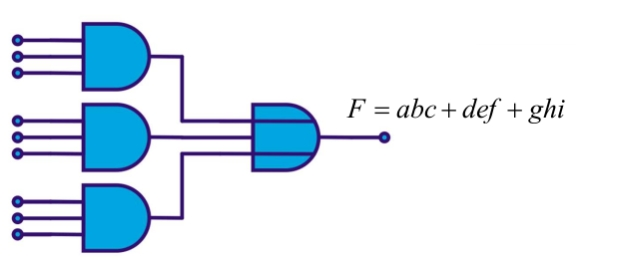
\includegraphics[width=10cm]{figures/ch13/combinatorial1.jpg}
	\caption{}
	\label{fig:combinatorial1}
\end{figure}

\begin{figure}[h!]
	\centering
	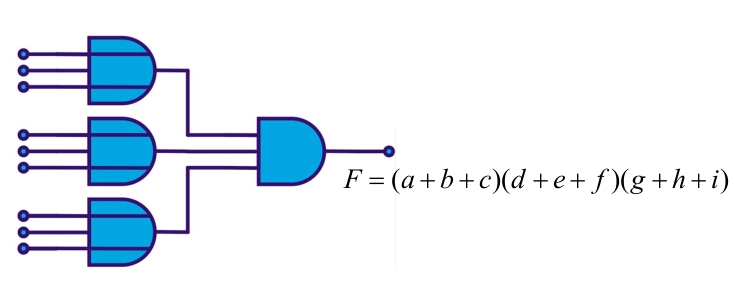
\includegraphics[width=12cm]{figures/ch13/combinatorial2.jpg}
	\caption{}
	\label{fig:combinatorial2}
\end{figure}

This is enough for implementation, but these circuits can be simplified by using only one type of logic gate. Any sum-of-products can also be implemented with only NAND-gates, as in figure \ref{fig:combinatorial3}, and a product-of-sums expression with only OR-gates.

\begin{figure}[h!]
	\centering
	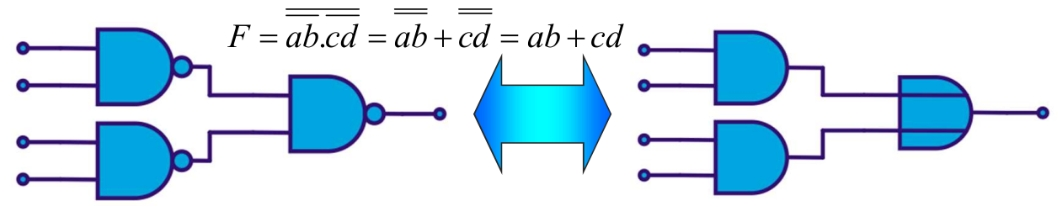
\includegraphics[width=12cm]{figures/ch13/combinatorial3.jpg}
	\caption{}
	\label{fig:combinatorial3}
\end{figure}

\begin{figure}[h!]
	\centering
	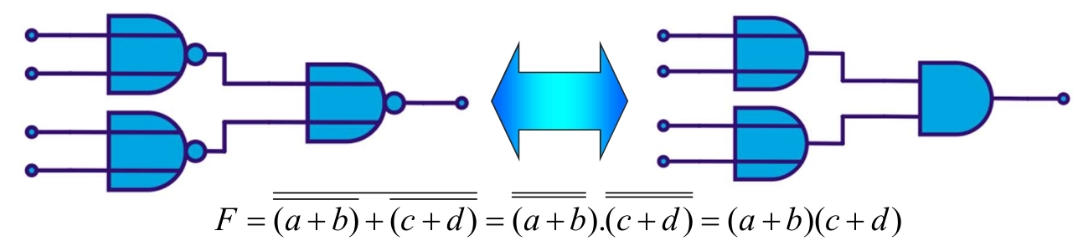
\includegraphics[width=12cm]{figures/ch13/combinatorial4.jpg}
	\caption{}
	\label{fig:combinatorial4}
\end{figure}


\subsection{Example: Digital Multiplexer}
\label{sec:multiplexer}
We apply this method to the design of a digital multiplexer. A digital multiplexer or \emph{MUX} is a device with $2$ inputs $A$ and $B$ and a selector $M$. The single output of the MUX is equal to $A$ if $M = 1$ and equal to $B$ if $M=0$. Its symbol is shown in figure \ref{fig:mux1}. The truth table can be trivially constructed from the description  and is represented in figure \ref{fig:mux2}. 

\begin{minipage}{.5\textwidth}
	\centering
	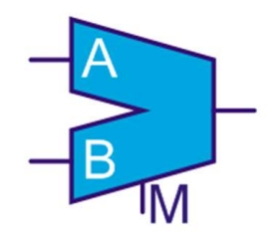
\includegraphics[width=5cm]{figures/ch13/mux1.jpg}
	\captionof{figure}{}
	\label{fig:mux1}
\end{minipage}%
\begin{minipage}{.5\textwidth}
	\centering
	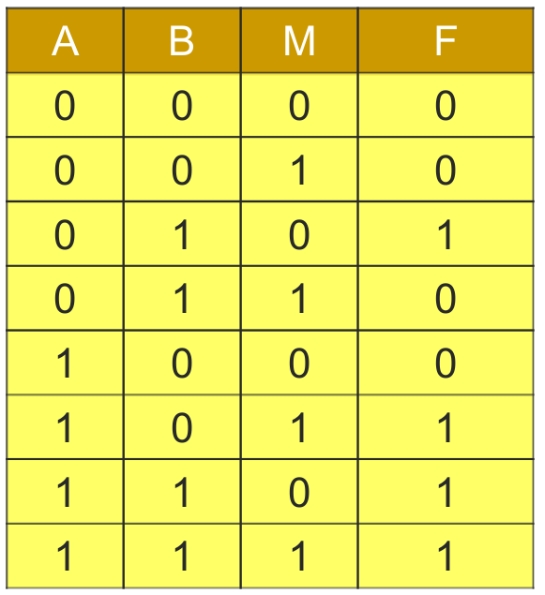
\includegraphics[width=4cm]{figures/ch13/mux2.jpg}
	\captionof{figure}{}
	\label{fig:mux2}
\end{minipage}
Based on the truth table, we can construct the sum-of-products:
\begin{align*}
	F &= \overline{A} \cdot B \cdot \overline{M} + A \cdot \overline{B} \cdot M + A \cdot B \cdot \overline{M} + A \cdot B \cdot M \\
	  &= \overline{A} \cdot B \cdot \overline{M} +  A \cdot B \cdot \overline{M}  + A \cdot \overline{B} \cdot M  + A \cdot B \cdot M \\	
	  &= (\overline{A} + A) \cdot B \cdot \overline{M} + (\overline{B} + B)  \cdot A \cdot M \\
	  &= B \cdot \overline{M} + \cdot A \cdot M \\
\end{align*}
because of the distributive property and $\overline{X} + X = 1$ for any $X$. It should be clear that simplifying these equations is important to reduce circuit complexity. We will see how we can do this reduction systematically in section \ref{sec:karnaugh}.\\
To implement the logic function, we need two AND-gates, one OR-gate and a NOT-gate to generate $\overline{M}$. The result is shown in figure \ref{fig:mux3}.

\begin{figure}[h!]
	\centering
	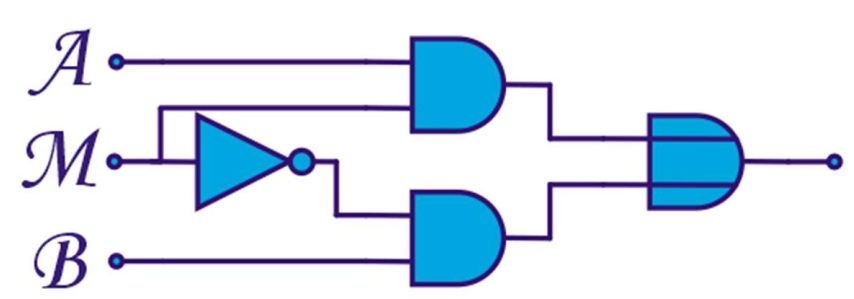
\includegraphics[width=10cm]{figures/ch13/mux3.jpg}
	\caption{}
	\label{fig:mux3}
\end{figure}

\section{CMOS Gates}
We already saw how we can make a NOT-gate from an NMOS and a PMOS transistor - see figure \ref{fig:not_gate}. To make a NAND- or NOR-gate, we need additional transistors to accept two input signals. How this is done in shown in figure \ref{fig:nand_gate} (NAND) and \ref{fig:nor_gate} (NOR).

\begin{minipage}{.5\textwidth}
	\centering
	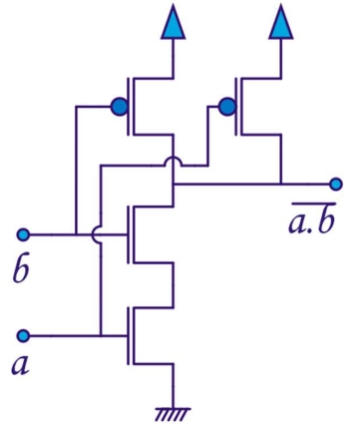
\includegraphics[width=5cm]{figures/ch13/nand_gate.jpg}
	\captionof{figure}{CMOS NAND Gate}
	\label{fig:nand_gate}
\end{minipage}%
\begin{minipage}{.5\textwidth}
	\centering
	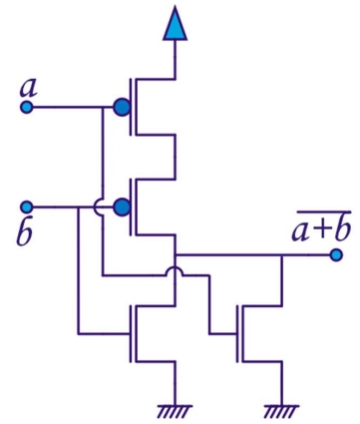
\includegraphics[width=5cm]{figures/ch13/nor_gate.jpg}
	\captionof{figure}{CMOS NOR Gate}
	\label{fig:nor_gate}
\end{minipage}

For the NAND-gate, the output is pulled to ground only when both inputs are high because then both NMOS in series will conduct. If at least one input is low, a PMOS in the top part will conduct and pull the output to the supply (high).\\
For the NOR-gate, the situation is reversed: if one input is high, the output is pulled to ground. If both are low, both PMOS in series conduct and the output is high.\\
The extension to more terminals is trivial, because it only requires the addition of more transistors, either in parallel or series with the existing transistors.\\
Note how these circuits have the same general structure: there are always two distinct blocks: the block on the top (with the PMOS transistors) is connected to the supply. When this block in total is closed the output is "1". If not, it is an open switch (high impedance). For the bottom part, containing the NMOS transistors, the situation is reversed: this part of the circuit generates the logic "0" because it can connect the output to ground. It is only a closed switch when the output is not "1", and an open switch otherwise. This means that both blocks have to be complementary. If this would not be the case, certain input configurations could create a conducting path between supply and ground.\\
\begin{figure}[h!]
	\centering
	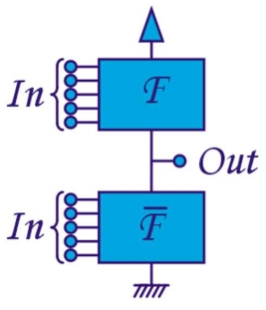
\includegraphics[width=4cm]{figures/ch13/cmos1.jpg}
	\caption{}
	\label{fig:cmos1}
\end{figure}
This duality is represented in figure \ref{fig:cmos1}, where the top block corresponds to $F = 1$, and the bottom block to $\overline{F} = 1 \Leftrightarrow F = 0$. For the NAND-gate:
\begin{itemize}
	\item p-block: $\overline{a} + \overline{b} = \overline{a \cdot b}$
	\item n-block: $a \cdot b$
\end{itemize}
And for the NOR-gate:
\begin{itemize}
	\item p-block: $\overline{a} \cdot \overline{b} = \overline{a + b}$
	\item n-block: $a + b$
\end{itemize}

This principle can be used to make gates of arbitrarily complexity. For instance, consider the XOR-gate we've seen before and which has the truth table in table \ref{table:xor}. The expression for the logic function is $F = \overline{a} \cdot b + a \cdot \overline{b}$.\\
\begin{table}
	\centering
	\begin{tabular}{|c|c|c|}
		\hline
		a & b  & $a\overline{b} + \overline{a}b$ \\
		\hline\hline
		0 & 0 & 0 \\
		\hline
		0 & 1 & 1 \\
		\hline
		1 & 0 & 1 \\
		\hline
		1 & 1 & 0 \\
		\hline
	\end{tabular}
\caption{}
\label{table:xor}
\end{table}
This expression for $F$ determines the p-block of the circuit, consisting of two branches in parallel, where each branch has two PMOS in series: $\overline{a} \cdot b$ and $a \cdot \overline{b}$.\\
To determine the n-block, we compute $\overline{F}$ by looking at the zero outputs: $\overline{F} = \overline{a} \cdot \overline{b} + a \cdot b$. This expression also leads to two parallel branches, each containing two NMOS in series, between output and ground. Both p- and n-blocks are implemented in figure \ref{fig:xor_gate}.

\begin{figure}[h!]
	\centering
	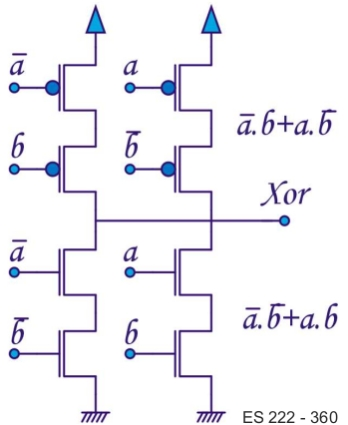
\includegraphics[width=6cm]{figures/ch13/xor_gate.jpg}
	\caption{}
	\label{fig:xor_gate}
\end{figure}

\subsection{Gate Inhibition}
\label{sec:inhibition}

It can be a problem when multiple gates are connected to the same point. For instance, consider the bus topology in figure \ref{fig:inhib1}, where multiple NAND-gates are connected to the same bus. If the output of one gate is high and the other gate is low, we have created a short-circuit between supply and ground. To avoid this, we add an extra input pin that allows to inhibit or deactivate the gate. Concretely, it will open the connections to both supply and ground, as in figure \ref{fig:inhib2} so the output is left dangling and its value is undetermined.

\begin{minipage}{.5\textwidth}
	\centering
	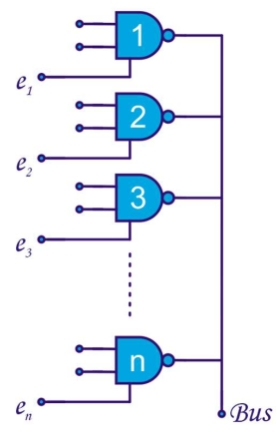
\includegraphics[height=6cm]{figures/ch13/inhib1.jpg}
	\captionof{figure}{}
	\label{fig:inhib1}
\end{minipage}%
\begin{minipage}{.5\textwidth}
	\centering
	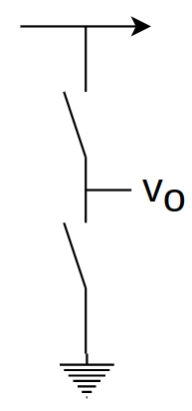
\includegraphics[height=4cm]{figures/ch13/inhib2.jpg}
	\captionof{figure}{}
	\label{fig:inhib2}
\end{minipage}

To implement this in CMOS, we put additional P- and NMOS-transistors between the output and respectively the upper and lower part, as in figure \ref{fig:inhib3}. The PMOS is driven by the inhibitor signal $e$ and the NMOS by $\overline{e}$. So if $e$ is high, both upper and lower parts are isolated from the output. This is \emph{active high} inhibition.

\begin{figure}[h!]
	\centering
	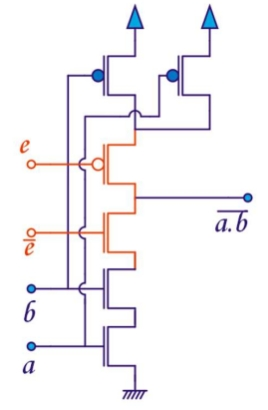
\includegraphics[height=7cm]{figures/ch13/inhib3.jpg}
	\caption{}
	\label{fig:inhib3}
\end{figure}


\section{Karnaugh Mapping}
\label{sec:karnaugh}

Any logic function $F$ can be uniquely defined with a truth table. However, the number of entries in this table depends exponentially on the number of inputs, as we've seen before. It is therefore imperative to not only obtain a logic expression from this table, but also to reduce this expression as much as possible before implementation. This reduces the number of components, and hence the complexity and chance of failure of the circuit.\\
A consistent way to reduce a boolean expression to a simpler form was proposed by Maurice Karnaugh in 1953. As an example, we consider a function of two variables:
$$F = a \overline{b} + a b + \overline{a}b$$
This function can be represented in a Karnaugh table, which is similar to the truth table we used before, but with the input variables rearranged in rows and columns. In figure \ref{fig:karnaugh1}, input $a$ is shown in the columns, input $b$ in the rows. The trick in the Karnaugh table is to group all outputs of the same kind ("0" or "1") in groups of size $2^k$, until all these similar outputs belong to at least one group. The goal is to choose these groups as large as possible. In the figure, we need $2$ groups of size $2^1$ to collect all the "1"s. Karnaugh shows that the expression can be reduced to $F = a + b$, because we find that $F = 1$ when either $a=1$ (group on the right) or if $b=1$ (group on the bottom).

\begin{minipage}{.4\textwidth}
	\centering
	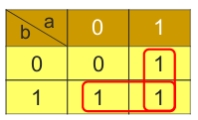
\includegraphics[width=3cm]{figures/ch13/karnaugh1.jpg}
	\captionof{figure}{}
	\label{fig:karnaugh1}
\end{minipage}%
\begin{minipage}{.5\textwidth}
	\centering
	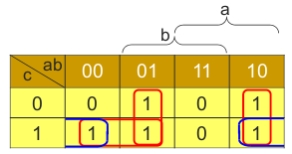
\includegraphics[width=5cm]{figures/ch13/karnaugh2.jpg}
	\captionof{figure}{}
	\label{fig:karnaugh2}
\end{minipage}

Could this simplification be achieved by symbolic manipulation? We could have grouped different terms in our expression:
$$
F = a \overline{b} + a b + \overline{a}b = a (\overline{b} + b ) + \overline{a} b = a + \overline{a} b
$$
but we can go no further in this way. But with the Karnaugh map, we see that we need to reuse a term ($ab$) to improve this result:
$$
F = a \overline{b} + a b + a b + \overline{a}b = a (\overline{b} + b ) + (\overline{a} + a) b = a + b
$$
In summary, the Karnaugh map shows us what terms to reuse, and with which other terms they should be recombined.\\
When we have three inputs, we group multiple inputs in a column, as in figure \ref{fig:karnaugh2}. It is important to write these inputs so that only a single bit changes from column to column - this is called a \emph{Grey code}. Once again, we group elements in groups of size $2^k$ - we find three different groups: $F = a \overline{b} + \overline{a} b + \overline{a} c$. Note that we could also have chosen another group: $F = a \overline{b} + \overline{a} b + \overline{b} c$.\\
If we have $4$ input variables, we encode them also in the rows - once again with a Grey code - and apply the exact same method. This is the example in figure \ref{fig:karnaugh3}, where the grouping already has been done. The result is $F = \overline{ab} + \overline{ac} +  \overline{ad} + bcd + \overline{bc} + \overline{bd}$.
\begin{figure}[h!]
	\centering
	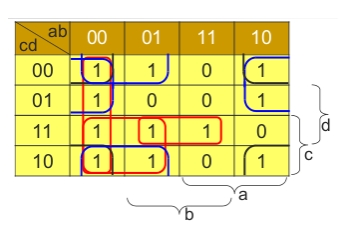
\includegraphics[width=6cm]{figures/ch13/karnaugh3.jpg}
	\caption{}
	\label{fig:karnaugh3}
\end{figure}
\\With more than $4$ variables, the visualization becomes harder. With $5$ variables, you can use two tables: one for the last variable $= 0$, and the other for $= 1$, but remember you'll have to group across tables. For many variables, you should use specialized software tools.

\subsection{Example: the Adder}

We now build a  digital circuit that adds two binary numbers $a$ and $b$. Furthermore, it can also accept a "carry in" $c_{in}$ so it can be used in a cascade of similar circuits that will form an adder. It has two outputs: the sum $s$ and the "carry out" $c_{out}$, as in figure \ref{fig:adder1}. The sum is $s = a \oplus b \oplus c_{in}$ with $\oplus$ the sum modulo $2$, and $c_{out} = \lfloor (a + b + c_{in}) / 2 \rfloor$. The results are summarized in the truth table in figure \ref{fig:adder2}. Since we have two outputs, we need to construct two Karnaugh tables: one for $c_{out}$, as in figure \ref{fig:adder3}, and one  for $s$ in figure \ref{fig:adder4}. The table for $c_{out}$ gives:
$$
c_{out} = a \cdot c_{in} + b  \cdot  c_{in} + a  \cdot b
$$
In the table for $s$, we find only groupings of size $1$, so $s$ can't be simplified beyond $$s = a \; \oplus  \;  b  \;  \oplus  \;  c_{in}$$.

\begin{minipage}{.4\textwidth}
	\centering
	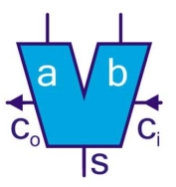
\includegraphics[width=4cm]{figures/ch13/adder1.jpg}
	\captionof{figure}{}
	\label{fig:adder1}
\end{minipage}%
\begin{minipage}{.5\textwidth}
	\centering
	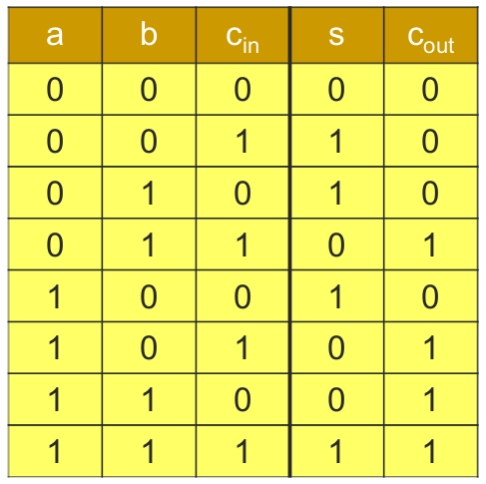
\includegraphics[width=5cm]{figures/ch13/adder2.jpg}
	\captionof{figure}{}
	\label{fig:adder2}
\end{minipage}

\begin{minipage}{.4\textwidth}
	\centering
	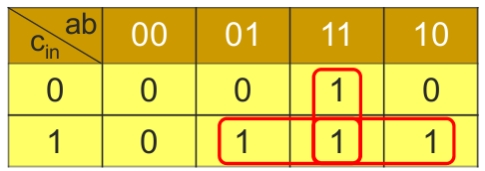
\includegraphics[width=6cm]{figures/ch13/adder3.jpg}
	\captionof{figure}{Table for $c_{out}$}
	\label{fig:adder3}
\end{minipage}%
\begin{minipage}{.5\textwidth}
	\centering
	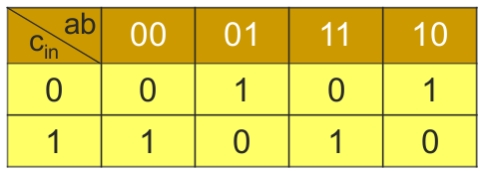
\includegraphics[width=6cm]{figures/ch13/adder4.jpg}
	\captionof{figure}{Table for $s$}
	\label{fig:adder4}
\end{minipage}

We implement $s$ with two XOR-gates, as in figure \ref{fig:adder5}. Output $c_{out}$ can be constructed with $4$ NAND-gates (confirm this) as in figure \ref{fig:adder6}.

\begin{minipage}{.5\textwidth}
	\centering
	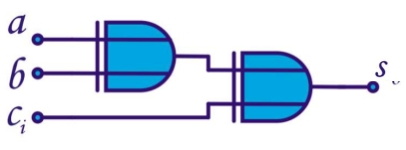
\includegraphics[width=7cm]{figures/ch13/adder6.jpg}
	\captionof{figure}{}
	\label{fig:adder5}
\end{minipage}%
\begin{minipage}{.5\textwidth}
	\centering
	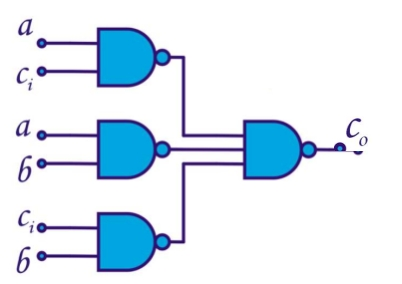
\includegraphics[width=7cm]{figures/ch13/adder5.jpg}
	\captionof{figure}{}
	\label{fig:adder6}
\end{minipage}

When we put multiple of these circuits in cascade, we get an adder. For example, to add $2$ $4$-digit binary numbers, we can use the circuit in figure \ref{fig:adder7} where the $c_{o}$ of one element is the $c_{i}$  of the next one. The carry in for the initial lowest bit is zero. If the sum can not be represented by a $4$-bit number, there will be an \emph{overflow} bit.\\
The circuit can also be used to subtract, because $b - a = b + (-a)$ and we can easily construct $-a$ with the two's-complement: for any binary $a = \sum_{i=0}^{n-1} b_i 2^i$:
$$-a = 2^n - \sum_{i=0}^{n-1} b_i 2^i = (1 + \sum_{i=0}^{n-1} 2^i) - \sum_{i=0}^{n-1} b_i 2^i = 1 + \sum_{i=0}^{n-1} (1-b_i) 2^i$$
So we construct $-a$ by inverting each bit and adding $1$, as in figure \ref{fig:adder8}, where the $1$ is added through the initial carry in.

\begin{minipage}{.5\textwidth}
	\centering
	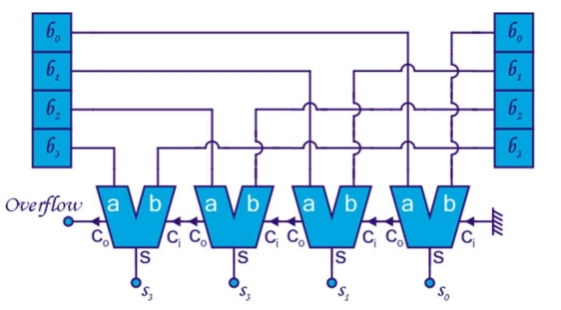
\includegraphics[width=7cm]{figures/ch13/adder7.jpg}
	\captionof{figure}{}
	\label{fig:adder7}
\end{minipage}%
\begin{minipage}{.5\textwidth}
	\centering
	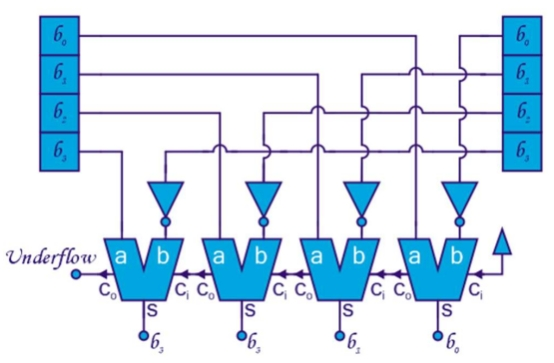
\includegraphics[width=7cm]{figures/ch13/adder8.jpg}
	\captionof{figure}{}
	\label{fig:adder8}
\end{minipage}

\chapter{Alternative Digital Families}
\label{ch:alternative}
In chapter \ref{ch:logic_gates}, we used Complementary MOS to implement the digital circuits. This is the predominant technology in use today. However, there are some applications that require specific digital technologies, mostly based on bipolar transistors. These technologies are much faster than CMOS.\\
In this chapter, we will discuss the most important of these BJT digital technologies: \emph{Transistor-Transistor Logic} or TTL, and ECL or \emph{Emitter-Coupled Logic}. At the end of the chapter, we'll also have a look at a special purpose circuit: the Schmidt trigger.

\section{BJT Logic Gate}
The first logic gates where implemented with bipolar transistors. A basic BJT circuit to implement a NOT-gate is seen in figure \ref{fig:rtl}. A high input voltage will generate a high base current through resistor $R_B$ and as a consequence, there will be a high collector current through $R$. The output $E - R\;I_C$ will be low. If the input is low, there will be no base or collector current and the output is high. This technology is also called \emph{Resistor-Transistor Logic} (RTL).\\
\begin{minipage}{.5\textwidth}
	\centering
	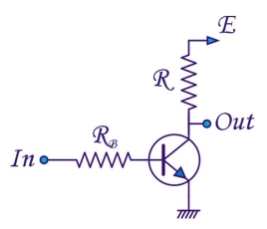
\includegraphics[width=5cm]{figures/ch15/rtl.jpg}
	\captionof{figure}{}
	\label{fig:rtl}
\end{minipage}%
\begin{minipage}{.5\textwidth}
	\centering
	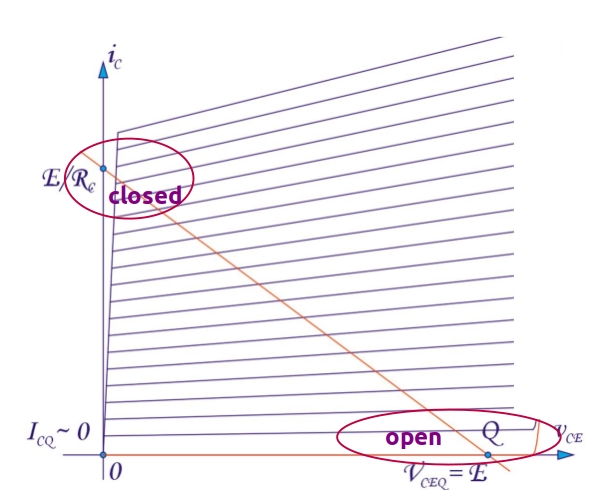
\includegraphics[width=7cm]{figures/ch15/rtl4.jpg}
	\captionof{figure}{}
	\label{fig:rtl4}
\end{minipage}

When the input is high ($\approx E$), there is lots of current and the transistor is in saturation and behaves as an closed switch. When the input is low ($\approx 0$), there is no base current, the transistor is in cut-off and behaves as an open switch - see figure \ref{fig:rtl4}. The input-output characteristic is seen in figure \ref{fig:rtl2} and is as expected.

\begin{minipage}{.5\textwidth}
	\centering
	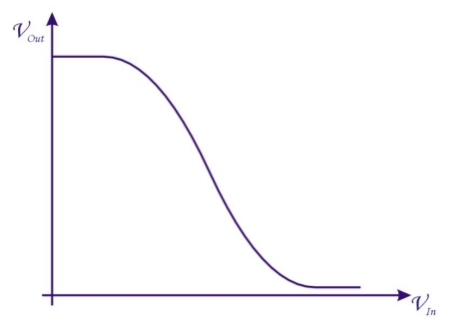
\includegraphics[width=7cm]{figures/ch15/rtl2.jpg}
	\captionof{figure}{}
	\label{fig:rtl2}
\end{minipage}%
\begin{minipage}{.5\textwidth}
	\centering
	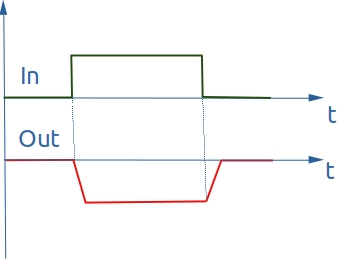
\includegraphics[width=7cm]{figures/ch15/rtl3.jpg}
	\captionof{figure}{}
	\label{fig:rtl3}
\end{minipage}

To analyze the dynamic behavior of the circuit, we need to take the capacitances at in- and output into account. This means that the output transient behavior doesn't follow the input immediately, but its speed is determined by the charging and discharging of the (parasitic) capacitance at rate $\frac{I}{C} t$ (for a constant current), as in figure \ref{fig:rtl3} with the slope of the output flanks $= \frac{I}{C}$. We need lots of current for a very fast gate.\\
The input capacitance is always present due to the junction capacitance $C$ between base and emitter. The current we can inject into the base is $I_B = \frac{E - V_{BEQ}}{R_E}$. This is the current available to charge $C$ and get a low output. To discharge, we need to put the input at ground, and the current is $I_B = \frac{V_{BEQ}}{R_E}$ to get a high output. This current is a lot lower than the charge current, what means that the gate goes very fast from 1 to 0, but very slowly from 0 to 1. To improve this behavior, we replace the resistor by a transistor.\\

\section{Transistor-Transistor Logic}
\label{sec:ttl}
By replacing the resistor by a transistor, we work with \emph{Transistor-Transistor Logic} (TTL). If the input in figure \ref{fig:ttl1} is low, the base-emitter junction of transistor \Circled{2} is forward biased because it sees a voltage $E$, and you will draw a current through the base via $R_B$: 
$$I_B = \frac{E - V_{BEQ}}{R_B} \text{ and } I_C = \beta \frac{E - V_{BEQ}}{R_B}$$
at least until the base capacitance is discharged. This current is lot higher than $\frac{V_{BEQ}}{R_E}$ we had in RTL. Transistor \Circled{1} from which we try to draw current from the base will block and the output is high.\\
When the input is high, we are in the peculiar situation where we are using the input transistor in inverted mode (see section \ref{sec:modes_of_operation}) where emitter and collector are interchanged. This means that between supply and ground we have two $V_{BEQ}$'s: once for the input transistor  \Circled{2} via $R_B$ and with the collector-base junction in forward bias, and between base and emitter of transistor \Circled{1}. The base current of transistor \Circled{2} is $\frac{E - 2V_{BEQ}}{R}$. While a transistor doesn't work as well in inverted mode, there is still current amplification (but with reduced $\beta$) so there is more than enough current available to charge the parasitic capacitance of transistor \Circled{1} and to polarize \Circled{1} in the saturation domain, leading to a low output.

\begin{minipage}{.5\textwidth}
	\centering
	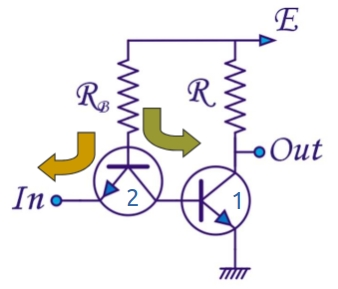
\includegraphics[width=7cm]{figures/ch15/ttl1.jpg}
	\captionof{figure}{}
	\label{fig:ttl1}
\end{minipage}%
\begin{minipage}{.5\textwidth}
	\centering
	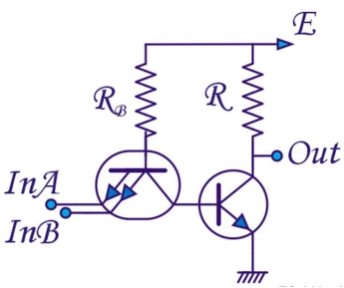
\includegraphics[width=7cm]{figures/ch15/ttl2.jpg}
	\captionof{figure}{}
	\label{fig:ttl2}
\end{minipage}

To create a NAND-gate, we replace transistor \Circled{2} with $2$ BJT transistors in parallel (i.e. base and collector at the same voltage) - as drawn in figure \ref{fig:ttl2}. The two emitters of these parallel input transistors will be the inputs. If one of the two inputs is low, its transistor will try to draw a current out of the base of the output transistor, such that this one will be in cut-off and the output is high. If both inputs are high, there is a large base current into the output transistor, so the output is low, as required.

\subsection{Totem-Pole Configuration}
The input transistor \Circled{2} in \ref{fig:rtl2} solved the issue with time difference between charging and discharging due to the input capacitance. We still have to deal with the output capacitance $C_L$ due to the load, as in figure \ref{fig:totem1}. This capacitor charges through resistor $R$ - with a time constant $R \; C_L$ - and discharges through  the BJT. The issue is that discharging via the BJT can happen a lot faster than charging via $R$.

\begin{minipage}{.5\textwidth}
	\centering
	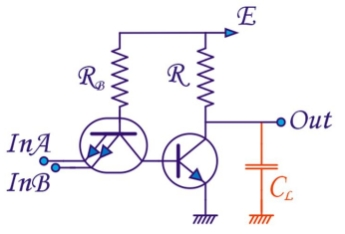
\includegraphics[width=7cm]{figures/ch15/totem1.jpg}
	\captionof{figure}{}
	\label{fig:totem1}
\end{minipage}%
\begin{minipage}{.5\textwidth}
	\centering
	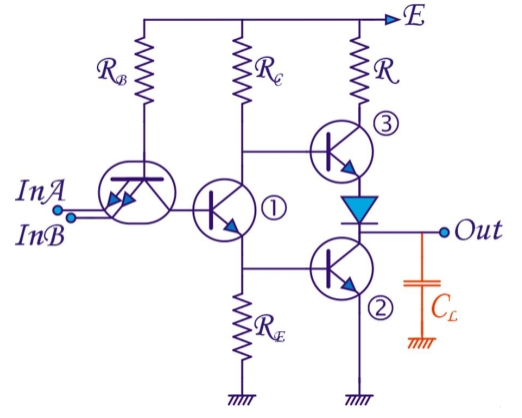
\includegraphics[width=7cm]{figures/ch15/totem2.jpg}
	\captionof{figure}{}
	\label{fig:totem2}
\end{minipage}

We improve this by:
\begin{itemize}
	\item Modifying the output stage by adding an emitter resistance $R_E$. This is now a phase-splitter.
	\item Adding an output stage with 2 BJT on top of each other. This is a \emph{totem-pole} configuration. The load capacitance $C_L$ will now charge through transistor \Circled{3} and discharge through transistor \Circled{2}.
\end{itemize}
With \Circled{1} operating as a phase splitter, we can relate the voltage variations at the bases of transistors \Circled{2} and \Circled{3}:
$$
\frac{v_{be3}}{v_{be2}} = -\frac{R_C}{R_E} \Leftrightarrow \frac{v_{be2}}{R_E} = -\frac{v_{be3}}{R_C}
$$

If an input is low, it tries to draw current from transistor \Circled{1} and $v_{B1}$ goes down, as in figure \ref{fig:totem_high}. Transistor \Circled{1} is an open switch and we can remove him for the analysis. because transistor \Circled{2} has $V_{BEQ} = 0$, it will block and \Circled{3} will saturate and conduct, so the output is high and $C_L$ charges through transistor \Circled{3}. However, the output is not equal to the supply $E$ - it is set via $R_C$ and the voltage drops over the base-emitter junction of \Circled{3} and the diode: $v_{OUT} = E - R_C I_B - V_{BEQ3} - V_{DQ} \approx E - 1.2V -R_C I_B$. Resistance $R_C$ can not be too high to reduce this voltage drop. For $E = 5$ V, the output will be $\approx 3.5$ V.

\begin{figure}[h!]
	\centering
	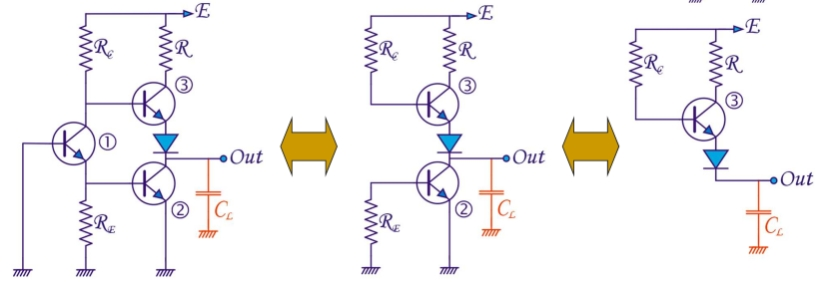
\includegraphics[width=16cm]{figures/ch15/totem_high.jpg}
	\caption{}
	\label{fig:totem_high}
\end{figure}

When both inputs are high, we can replace their base-collector junction by a forward-biased diode, as in figure \ref{fig:totem_low}. Transistor \Circled{1} is saturated and we can replace it by a voltage source $V_{CE,Sat}$. This means that $V_{B3} = V_{BEQ2} + V_{CE,Sat1} \approx 0.8$ V. Resistance $R_E$ is chosen such that $V_{BE2} = (E - V_{CE,Sat}) \frac{R_E}{R_E + R_C} \approx 0.8$ V. Consequently $V_{BE3} = V_{B3} - V_{E3} = V_{BEQ2} + V_{CE,Sat1} - (V_{CE,Sat2+V_{DQ}}) \approx 0$. So transistor \Circled{2} is saturated and \Circled{3} is blocked. This is also why the diode is there: to make sure that \Circled{3} is blocked when \Circled{2} is saturated. The minimum output voltage that corresponds to a low signal is $V_{CE,Sat2} \approx 0.2$ V.

\begin{figure}[h!]
	\centering
	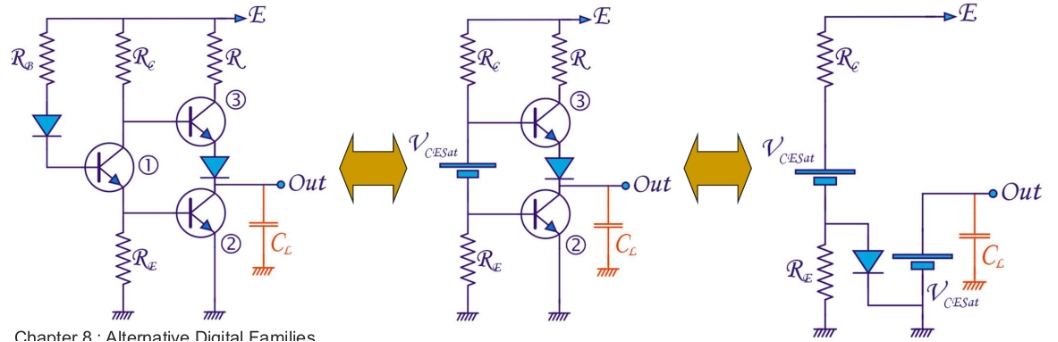
\includegraphics[width=16cm]{figures/ch15/totem_low.jpg}
	\caption{}
	\label{fig:totem_low}
\end{figure}

When a transistor turns on, we provide a lot of base current in TTL, more base current than it needs for the collector current it is drawing - the transistor is saturated. The extra base current creates a stored charge in the base of the transistor. As discussed, this stored charge causes problems when the transistor needs to be switched from on to off: while the charge is present, the transistor is on; all the charge must be removed before the transistor will turn off. Removing the charge takes time, so the result of saturation is a delay between the applied turn-off input at the base and the voltage swing at the collector. To avoid that the transistor saturates, we place a Schottky diode with a threshold voltage of $0.3$ V between base an collector (figure \ref{fig:schottky_transistor}). By doing so, the collector-emitter voltage $V_{CE} = V_{BEQ} - 0.3V = 0.3V  > V_{CE, Sat}$ and the transistor can never saturate. 

\begin{figure}[h!]
	\centering
	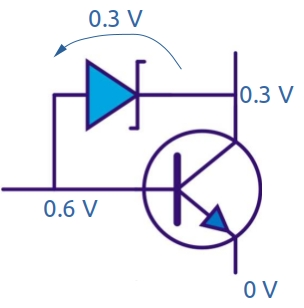
\includegraphics[width=5cm]{figures/ch15/schottky_transistor.jpg}
	\caption{A Schottky transistor}
	\label{fig:schottky_transistor}
\end{figure}



\section{Emitter-Coupled Logic}
\label{sec:ecl}
Transistor-Transistor logic is based on the saturation and blocking of the bipolar transistor (figure \ref{fig:rtl4}). This means that there will be large voltage swings and several crucial circuit node have to be charged and discharged. That's why TTL is inherently slow (but still faster than CMOS). \emph{Emitter-Coupled Logic} (ECL) is  faster because the transistors never saturate and the voltage swings are kept low ($\sim \pm 400 mV$). The technology is also called \emph{Current Mode Logic} (CML). It is based on a differential topology, as in the differential amplifier from chapter \ref{sec:diff_amplifier} where two input transistors share the emitter node.\\
A typical ECL NOT-gate is shown in figure \ref{fig:ecl1}. The true gate is the differential amplifier in blue. The two common-collector amplifiers in red are just there shift the outputs one $V_{BEQ}$ lower and to buffer the outputs voltages because they provide a low output impedance.  Note that one input transistor is put at a reference voltage $V_{ref}$. The other transistor provides the input.\\
When $V_a > V_{ref}$, all current $I_{CC}$ will flow through the left branch. So the collector voltage $V_{C1} = E-R\;I_{CC}$ will be low and $V_{C2} = E$ will be high. We will assume that the input voltage is high when $V_a = V_{ref} + \frac{1}{2} V_{BEQ}$ and low when $V_a = V_{ref} - \frac{1}{2} V_{BEQ}$.
At the output, we then have:
\begin{itemize}
	\item HIGH $= E - V_{BEQ}$
	\item LOW $= E - R\;I_{CC} - V_{BEQ}$
\end{itemize}
\begin{figure}[h!]
	\centering
	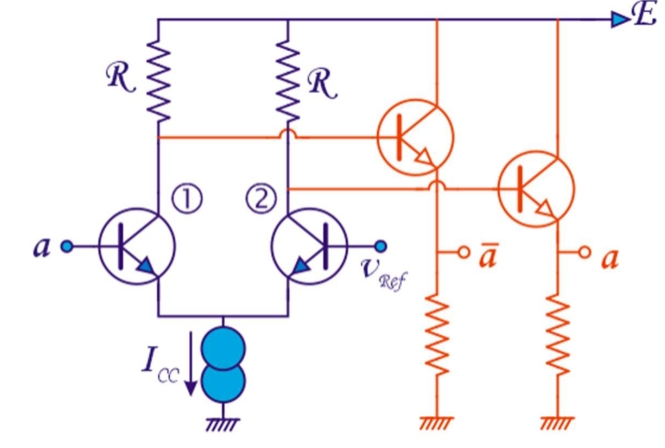
\includegraphics[width=10cm]{figures/ch15/ecl1.jpg}
	\caption{}
	\label{fig:ecl1}
\end{figure}
The difference between high and low (the output swing) is thus $R\;I_{CC}$ and must be equal to $V_{BEQ}$ because this is the swing at the input. So, this means that:
\begin{itemize}
	\item HIGH $= E - V_{BEQ}$
	\item LOW $= E -  2 V_{BEQ}$
\end{itemize}
And the reference value must be halfway between HIGH and LOW: $V_{ref} = \frac{V_{HIGH} + V_{LOW}}{2} = E - \frac{3}{2} V_{BEQ}$. Note that the ECL-gate always has two complementary outputs. Furthermore, the transistor never saturates because $V_{CE, min} = V_{BEQ}$. This is because when $V_a = V_{ref} + \frac{1}{2} V_{BEQ}$, $V_{C1} = E-V_{BEQ}$ and $V_{E1} =  V_{ref} - \frac{1}{2} V_{BEQ} = E - 2V_{BEQ}$, so $V_{CE1} = V_{BEQ} > V_{CE, Sat}$. This is even more valid for the other transistor, because his collector voltage is $E$, so $V_{CE} = 2V_{BEQ} > V_{CE, Sat}$. \\

\subsection{NOR Gate}

When we want to create a NOR-gate, it is enough to add a transistor in parallel with the existing input transistor, as in figure \ref{fig:ecl2}. If one of the inputs is HIGH, that branch will conduct (regardless of what happens with the other input) and there will be a voltage drop across $R$ such that the voltage in the left node will be LOW. The other branch automatically offers $a \text{ OR } b = a + b$.

\begin{figure}[h!]
	\centering
	\includegraphics[width=8cm]{figures/ch15/ecl2.jpg}
	\caption{}
	\label{fig:ecl2}
\end{figure}

\subsection{NAND Gate}

To implement a NAND-gate, you would add a transistor in series with the existing input transistor. In that case, there's only conduction in the left branch - and also a low voltage - when both inputs are high. However, the issue is that both inputs are not on the same level because the transistors are stacked. So we compare $a - V_{BEQ}$ with $V_{ref} - V_{BEQ}$ instead of comparing $a$ with $V_{BEQ}$. Sa $a$ is level-shifted down with one $V_{BEQ}$ with the transistor to which $a$ is connected.

\begin{figure}[h!]
	\centering
	\includegraphics[width=8cm]{figures/ch15/ecl3.jpg}
	\caption{}
	\label{fig:ecl3}
\end{figure}


\section{The Schmidt Trigger}
\label{sec:schmidt}
% video 24 - 25:07
A digital signal gets corrupted by noise, as in figure \ref{fig:schmidt1}. Suppose you want to reconstruct the original signal. Conceptually, this should be simple: just use a comparator with a hard threshold (i.e. an OPAMP with no feedback and $v^- = v_{treshold}$) as in figure \ref{fig:schmidt2} where $v_{threshold}$ is midway between a LOW and HIGH voltage, and you should be able to remove the noise. However, as figure \ref{fig:schmidt3} demonstrates, this is not the case: the amplitude noise is transformed in phase noise, and the reconstructed signal is useless.

\begin{minipage}{.5\textwidth}
	\centering
	\includegraphics[width=8cm]{figures/ch15/schmidt1.jpg}
	\captionof{figure}{}
	\label{fig:schmidt1}
\end{minipage}%
\begin{minipage}{.5\textwidth}
	\centering
	\includegraphics[width=6cm]{figures/ch15/schmidt2.jpg}
	\captionof{figure}{}
	\label{fig:schmidt2}
\end{minipage}

\begin{figure}[h!]
	\centering
	\includegraphics[width=16cm]{figures/ch15/schmidt3.jpg}
	\caption{}
	\label{fig:schmidt3}
\end{figure}

A better way to recover the original signal, is by using \emph{hysteresis} - as shown in figure \ref{fig:schmidt4}: a signal value is classified as HIGH when the voltage is higher than $v_h$. The signal will remain HIGH until it falls below a voltage $v_l < v_h$, when it will be considered as LOW. It will only return to being HIGH when $v_o > v_h$. When we apply this hysteresis comparator to the noisy signal, we can reconstruct the underlying signal perfectly, as figure \ref{fig:schmidt5} demonstrates.

\begin{minipage}{.5\textwidth}
	\centering
	\includegraphics[width=7cm]{figures/ch15/schmidt4.jpg}
	\captionof{figure}{}
	\label{fig:schmidt4}
\end{minipage}%
\begin{minipage}{.5\textwidth}
	\centering
	\includegraphics[width=8cm]{figures/ch15/schmidt6.jpg}
	\captionof{figure}{}
	\label{fig:schmidt6}
\end{minipage}

\begin{figure}[h!]
	\centering
	\includegraphics[width=16cm]{figures/ch15/schmidt5.jpg}
	\caption{}
	\label{fig:schmidt5}
\end{figure}

To implement a comparator with hysteresis, we use a Schmidt trigger: an OPAMP with feedback on the positive node, as in figure \ref{fig:schmidt6}, so it is unstable. Note that we already used this device in the fantastron oscillator from chapter \ref{ch:fantastron} but we will study it in more detail in this section.\\
At the positive node, we can write:
\begin{align}
	v_{ref} + v &= \frac{v_i/R_1 + v_o/R_2}{1/R_1 + 1/R_2}\\
				&= \frac{\frac{R_2}{R_1} v_i + v_o}{1 + R_2/R_1} \\
				&= \frac{k v_i + v_o}{1+k} \\
	v_o &= (1+k) \; v_{ref} + (1+k) \; v - k v_i
	\label{eq:schmidt1}
\end{align}
We can plot this line on the $v_o - v$ characteristic of the OPAMP: $v_o = \Phi(v)$, as in figure \ref{fig:schmidt7}. The diagonal line that represents equation \ref{eq:schmidt1} moves horizontally with varying input voltage $v_i$. The intersection of this line with $\Phi(v)$ provides at maximum $3$ solutions. The method of Lyapounov allows us to check the stability of these nodes by linearizing $\Phi$ around them: $v_o = A \; v$ with $A$ very large in the middle and $\approx 0$ when $v_o = \pm E$. If we work with a fixed $v_i$ and fixed $v_{ref}$, we can also write \ref{eq:schmidt1} around the operating point:
\begin{align}
	v_o &= (1+k) \; v
	\label{eq:schmidt1_lin}
\end{align}
\begin{figure}[h!]
	\centering
	\includegraphics[width=7cm]{figures/ch15/schmidt7.jpg}
	\caption{}
	\label{fig:schmidt7}
\end{figure}
With the OPAMP as a low-pass first-order system, the gain is 
$$v_o = \frac{A_0}{1 + sT}$$
Substituting this in equation \ref{eq:schmidt1_lin}, we get:
\begin{align*}
	A_0 v_o = (1 + k)v + sT (1+k) v &= (1+k)v + T(1+k) \frac{d}{dt} v \\
	\Rightarrow \frac{d}{dt} v &= \frac{A_0 - (1+k)}{T(1+k)} v
\end{align*}
So the circuit is stable when 
$$A_0 - (1+k) < 0 \Leftrightarrow A_0 < 1 + k$$
The system is stable in the operating points where $v_o = \pm E$ and unstable in the middle. This means that if the operating point ends up in the middle where $A_0$ is high, it will return to one of the two stable operating points after some time.\\
When $v_i$ is high, the diagonal line lies to the right, and there is only one intersection with $\Phi$, namely when $v_o = E$, and this point is stable. As $v_i$ decreases, there will come a point when there is also an intersection with the lower part of $\Phi$, namely when $v = 0$ with $v_o = E$, i.e.:
$$v = 0 \Rightarrow v_o = (1+k)v_{ref} - kv_i \Rightarrow v_i = \frac{R_1}{R_2} E + (1 + \frac{R_1}{R2}) v_{ref}$$
From that point one there are $3$ intersections, but the operating point remains on $v_o = E$ because this point is stable. When $v_i = -\frac{R_1}{R_2} E + (1 + \frac{R_1}{R2}) v_{ref}$, the top operating point disappears because there is no longer an intersection with $v_o = E$ and the operating must move to the only remaining (stable) operating point , namely $v_o = -E$. When $v_i$ starts to increase, the output remains equal to $-E$ as long as this point exists as a fixed point, only to switch to $v_o = E$ when it disappears. This cycle is represented in figure \ref{fig:schmidt8}.\\
\begin{minipage}{.5\textwidth}
	\centering
	\includegraphics[width=7cm]{figures/ch15/schmidt8.jpg}
	\captionof{figure}{}
	\label{fig:schmidt8}
\end{minipage}%
\begin{minipage}{.5\textwidth}
	\centering
	\includegraphics[width=8cm]{figures/ch15/schmidt9.jpg}
	\captionof{figure}{}
	\label{fig:schmidt9}
\end{minipage}
So we have created a hysteresis comparator with 
$$v_l = -\frac{R_1}{R_2} E + \bigg( 1 + \frac{R_1}{R2} \bigg) v_{ref}  \text{ and } v_h = \frac{R_1}{R_2} E + \bigg(1 + \frac{R_1}{R2} \bigg) v_{ref}$$
as in figure \ref{fig:schmidt9}. The trip point is $(1 + \frac{R_1}{R_2})\; v_{ref}$ and the hysteresis is $2\frac{R_1}{R_2} \; E$. We can use $v_{ref}$ to set the trip point and $\frac{R_1}{R_2}$ to determine the hysteresis.\\
The symbol of this gate is represented in figure \ref{fig:schmidt10}.
\begin{figure}[h!]
	\centering
	\includegraphics[width=9cm]{figures/ch15/schmidt10.jpg}
	\caption{}
	\label{fig:schmidt10}
\end{figure}

\chapter{Digital Circuit Implementation}
\section{Field-Programmable Gate Array}
A field-programmable gate array (FPGA) is an integrated circuit that can be programmed and reprogrammed to perform a specific function or task. Unlike traditional application-specific integrated circuits (ASICs), which are designed for a specific purpose and cannot be modified after manufacturing, FPGAs are designed to be flexible and can be reconfigured or programmed by the user to perform a variety of tasks.

FPGAs consist of programmable logic blocks and interconnects that can be configured to create custom digital circuits. The programmable logic blocks can be configured to perform basic logic functions such as AND, OR, and XOR gates, and the interconnects allow these blocks to be connected to create more complex circuits.

FPGAs are commonly used in a variety of applications, including digital signal processing, image and video processing, networking, and aerospace and defense systems. They offer high performance, low power consumption, and flexibility, making them a popular choice for many types of applications.

\section{Programmable Logic Array}
A programmable logic array (PLA) is a type of digital logic device that is used to implement combinational logic circuits. It consists of an array of AND gates, followed by an array of OR gates. The inputs to the AND gates are programmable, meaning that they can be configured to take on any combination of values. The outputs of the AND gates are then fed into the OR gates, which produce the final output.

The configuration of the inputs to the AND gates is typically stored in non-volatile memory such as ROM or EEPROM, allowing the circuit to be programmed to perform a specific function. Once programmed, the circuit can be used to implement a wide range of digital logic functions, including Boolean logic, arithmetic operations, and data manipulation.

PLAs are a type of field-programmable logic device (FPLD), which are used to implement custom digital logic circuits without the need for custom-designed integrated circuits. While PLAs are not as flexible as FPGAs, they offer a simpler and more cost-effective solution for many applications. They are commonly used in industrial control systems, automotive applications, and telecommunications equipment.

\section{Hardware Description Languages}

A hardware description language (HDL) is a specialized programming language used to design and describe digital circuits and systems. HDLs allow designers to create complex digital circuits by describing their behavior using a high-level language, rather than manually designing the circuit at the gate or transistor level.

VHDL (VHSIC Hardware Description Language) is one of the most commonly used HDLs. It was developed by the U.S. Department of Defense in the 1980s as part of the VHSIC (Very High-Speed Integrated Circuit) program. VHDL is a powerful language that can be used to describe the behavior of digital systems at multiple levels of abstraction, from the lowest level of gates and transistors to the highest level of system behavior.

In VHDL, digital circuits are described using entities, which represent the interface and behavior of a particular module, and architectures, which define the internal structure and behavior of the module. VHDL provides a wide range of constructs for describing the behavior of digital circuits, including conditional statements, loops, and procedures, as well as support for data types, signals, and ports.

VHDL is used extensively in the design and verification of digital systems, including ASICs, FPGAs, and other types of digital circuits. It is supported by a wide range of software tools, including simulators, synthesis tools, and verification tools, which allow designers to simulate, test, and verify their designs before they are implemented in hardware.
 